\documentclass{scrartcl}
\usepackage[utf8]{inputenc}
\usepackage[english]{babel}
\usepackage{caption}
\usepackage{subcaption}
\usepackage{listings}
\usepackage{pdfpages}
\usepackage{amsmath,amssymb}
\usepackage{siunitx}
\usepackage{hyperref}
\usepackage{mhchem}
\usepackage[section]{placeins}
\usepackage[activate, protrusion=true, expansion=true]{microtype}
\usepackage[left=2.5cm, right=2.5cm, bottom=2.5cm, top=2.5cm]{geometry}
\usepackage{libertine}
\usepackage{longtable}

\definecolor{mygreen}{rgb}{0,0.6,0}
\definecolor{mymauve}{rgb}{0.58,0,0.82}
\definecolor{mygray}{rgb}{0.5,0.5,0.5}
\lstset{backgroundcolor=\color{white},
  keepspaces=true,
  captionpos=b,
  keywordstyle=\color{blue},
  language=matlab,
  stringstyle=\color{mymauve},
  tabsize=2,
  numbers=left,                    % where to put the line-numbers; possible values are (none, left, right)
  numbersep=5pt,                   % how far the line-numbers are from the code
  numberstyle=\tiny\color{mygray},
  basicstyle=\footnotesize,        % the size of the fonts that are used for the code
  breakatwhitespace=false,         % sets if automatic breaks should only happen at whitespace
  breaklines=true,                 % sets automatic line breaking
  commentstyle=\color{mygreen},    % comment style
  deletekeywords={input},            % if you want to delete keywords from the given language
}

\newcommand*{\matlabcode}[3]{\begin{figure}[h!]\lstinputlisting[caption=#2, label=#3]{#1}\end{figure}}


\usepackage{scrpage2}
\pagestyle{scrheadings}
\automark{section}
\ihead{\rightmark}
\chead{}
\ohead{
\includegraphics[scale=0.025]{figures/EPFL_Logo.png}}
\setheadsepline{.4pt}

\begin{document}

\begin{titlepage}

\title{CE-1: Nonparametric Methods} % Title
\author{Arne Sachtler \\ Julia Krottenthaler}		% Author
\date{\today}								% Date

\makeatletter
\let\thetitle\@title
\let\theauthor\@author
\let\thedate\@date
\makeatother

\centering
\vspace*{0.5 cm}

    
\includegraphics[width=0.7\linewidth]{figures/EPFL_Logo.png}\\[1.0 cm]	
	\textsc{\Large System Identification (ME-421)}\\[1.0cm]				
	\rule{\linewidth}{0.2 mm} \\[0.5 cm]
	{ \LARGE \thetitle}\\
	\rule{\linewidth}{0.2 mm} \\[1.5 cm]
	
    \vspace{1cm}
	\begin{minipage}{0.5\textwidth}
		\begin{flushleft} \large
			\emph{{Students}:}\\
			\theauthor
			\end{flushleft}
			\end{minipage}~
			\begin{minipage}{0.4\textwidth}
			\begin{flushright} \large
			\emph{{Lecturer}:} \\	
			Prof. Karimi Alireza  \\
		\end{flushright}
	\end{minipage}\\[1.2cm]
	{\vspace{3cm} \large Lausanne, \thedate}\\[1.5 cm]
	\vfill
\end{titlepage}

%\newpage
\section{Step Response}
Figure~\ref{fig:testmodel} shows the modeled system, which will be used for the system identification exercises and
Figure~\ref{fig:responses} shows the step and impulse response for the system. 
\begin{figure}[h]
	\centering
	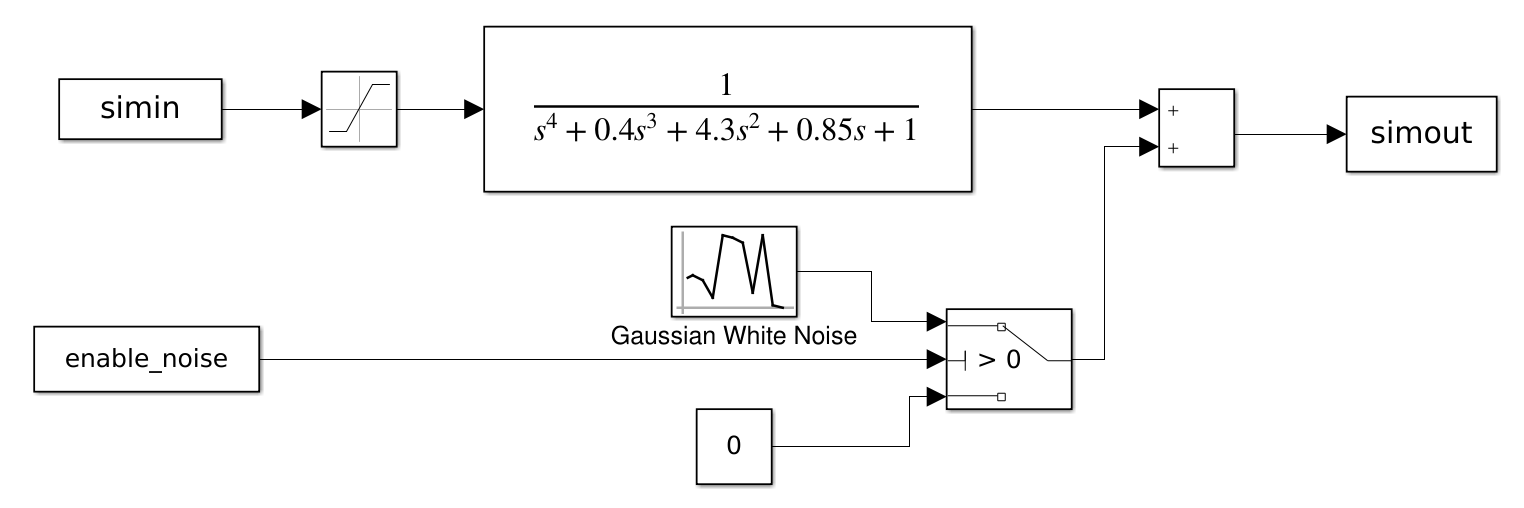
\includegraphics[height=5cm]{figures/systemmodel.png}
	\caption{Simulink model of the test system. We can enable or disable the noise setting the variable \texttt{enable\_noise} externally.}\label{fig:testmodel}
\end{figure}
\begin{figure}[h]
	\centering
	\begin{subfigure}{0.49\textwidth}
		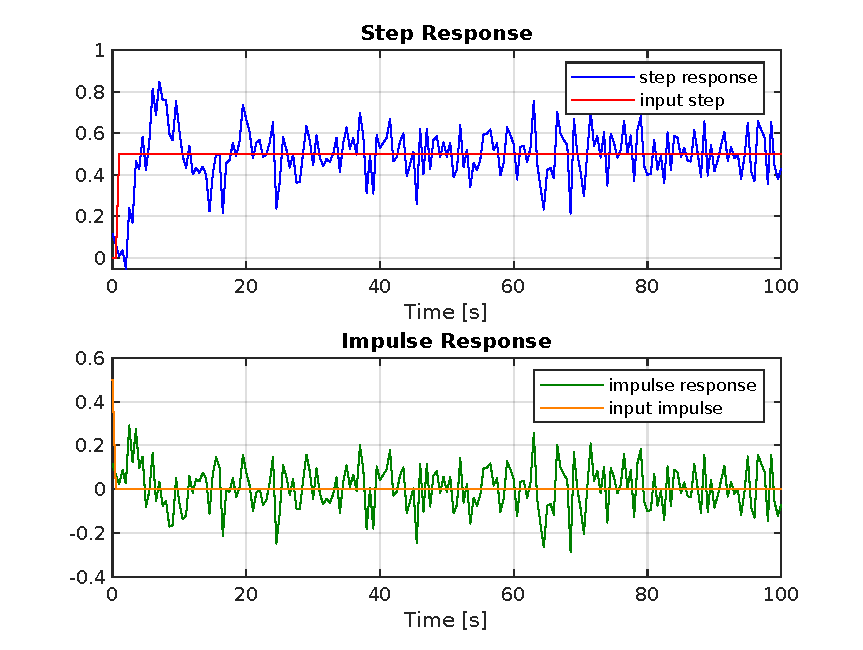
\includegraphics[width=.8\textwidth]{figures/noisy_responses.pdf}
		\subcaption{Noisy responses}
	\end{subfigure}
	\begin{subfigure}{0.49\textwidth}
		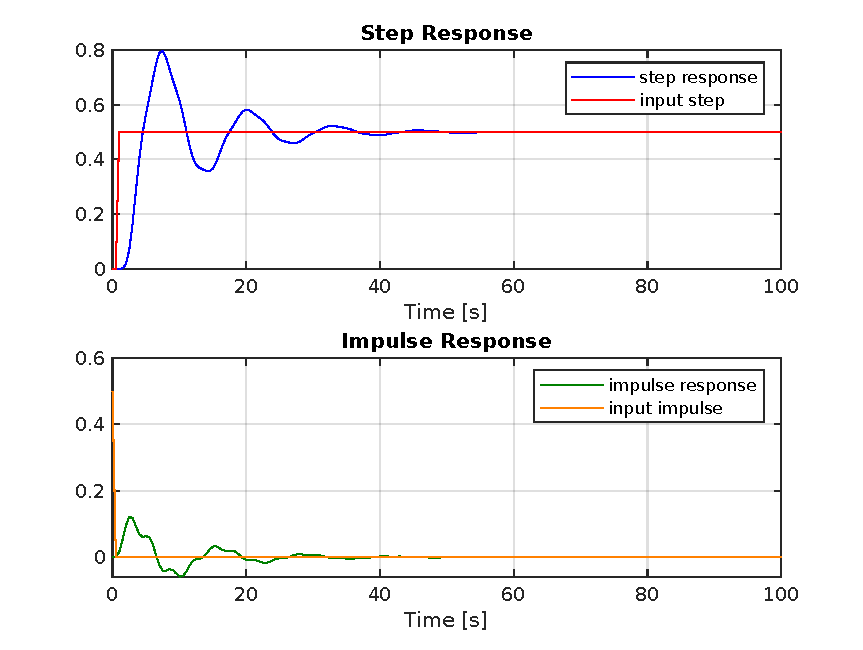
\includegraphics[width=.8\textwidth]{figures/noisefree.pdf}
		\subcaption{Responses without noise}
	\end{subfigure}
	\caption{Step and impulse responses of the test system with and without noise. Note, that we do not show unit step- and impulse responses, but scaled versions.}\label{fig:responses}
\end{figure}

\paragraph{Choice of the sampling period: } 
Factoring the poles of the system shows the poles $s_{1,2} \approx -0.1 \pm 2j$ and $s_{3,4} \approx -0.099 \pm 0.489j$. 
Neglecting the small real part, we approximately have resonances at $\omega_1 \approx 2 \frac{rad}{s}$ and $\omega_2 \approx 0.5 \frac{rad}{s}$.
The sampling frequency $\omega_{s} = 0.5 \cdot 2\pi \frac{rad}{s} = \pi \frac{rad}{s}$ is significantly larger than the higher resonance frequency.
The bode diagram of the transfer function shows a damping of $\approx -35dB$ at the sampling frequency.
As the signals in region hide in the noise anyway, we believe the sampling period of $T_e = 0.5s$ is a reasonable choice.
\paragraph{Comment on the scale of the impulse response: }
We apply an discrete-time impulse with a magnitude of $u(k) = 0.5\delta(k)$ where $\delta(k)$ denotes the Kronecker delta.
Due to the saturation block in the system, we can not apply a higher impulse signal without exciting nonlinearities of the model.
Consequently, the impulse response resulting from the experiment of applying $u(k)$ is only half the true unit impulse response of the system.
The impulse response estimation methods used later, all identify the impulse response to a unit impulse applied to the system.
Therefore, in order to get a unit impulse response, the impulse response obtained by the simulation of the SIMULINK model need to by scaled up by a factor of two.
The same arguments apply to the step response.

\newpage
\section{Auto Correlation of a PRBS signal}
In order to compute the cross-correlation of two discrete-time signals $u(k)$ and $y(k)$, we use 
\begin{equation}
	R_{uy}(h) = \frac{1}{M} \sum\limits_{k=0}^{M-1} u(k)y(k-h)\, .
\end{equation}
We assume two equal-length vectors for the signals $u$ and $y$. Let the length of the input signals be $N$, we choose the following interval for $h$
\begin{equation}
	h \in \{-H, \dots, -1, 0, 1, \dots, H\}\text{ , where } H = \left\lceil \frac{N}{2} \right\rceil \, .
\end{equation}
Using these definitions the cross-correlation can be computed in MATLAB using the code snippet shown in Listing~\ref{lst:corr}.

\matlabcode{../matlab/ce1/intcor.m}{Computing a discrete-time cross correlation of the signal u and y in MATLAB}{lst:corr}

In order to validate our implementation of the cross-correlation function, we use it to compute the autocorrelation two different test signals. 
Figure~\ref{fig:autocorr} shows the autocorrelation function of two different types of signals. 
On the left hand side (Figure~\ref{fig:autocorrPRBS}) there is a PRBS signal (length of the shift register is 4 and number of periods is 2) and its corresponding autocorrelation function. 
In addition, the figure on the right hand side (Figure~\ref{fig:autocorrSINUS}) displays a sinusoidal signal and its autocorrelation function.  

\begin{figure}[h]
	\centering
	\begin{subfigure}{0.45\textwidth}
		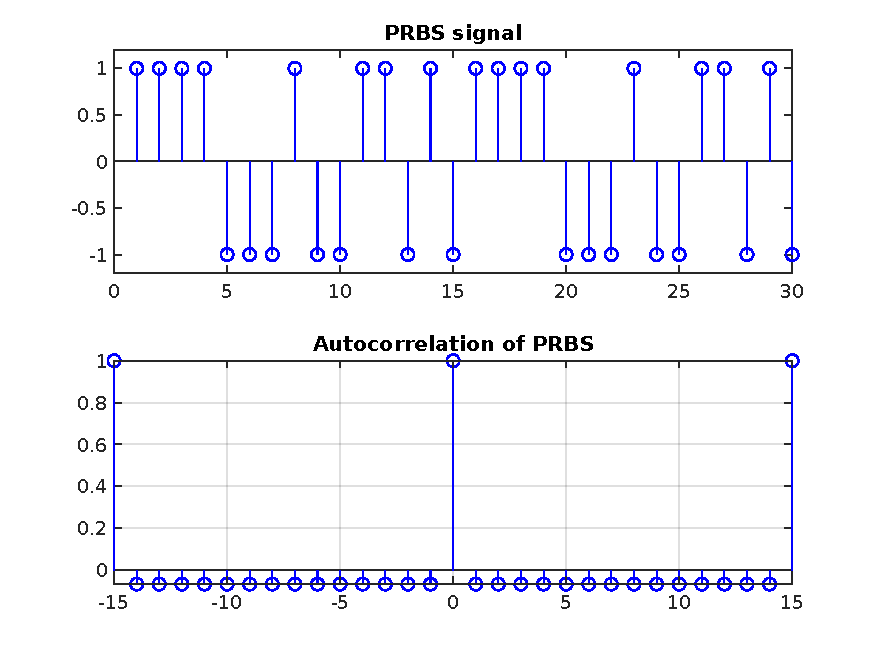
\includegraphics[width=\textwidth]{figures/prbs.pdf}
		\subcaption{PRBS signal}
		\label{fig:autocorrPRBS}
	\end{subfigure}
	\begin{subfigure}{0.45\textwidth}
		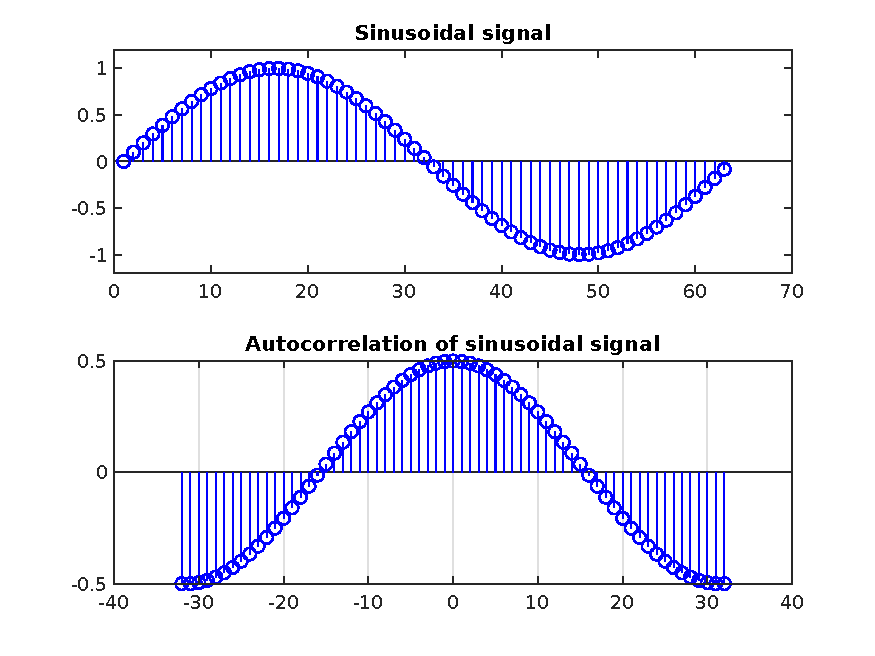
\includegraphics[width=\textwidth]{figures/sine.pdf}
		\subcaption{Sinus signal}
		\label{fig:autocorrSINUS}
	\end{subfigure}
	\caption{Two signals and their corresponding autocorrelation function}\label{fig:autocorr}
\end{figure}


\newpage
\section{Impulse Response using the Deconvolution Method}\label{section:numdec}
In this exercise the deconvolution method is used in order to estimate the impulse response of a system.
We use a digital random white noise signal, feed it to the model and record the system's response.
As an input signal we generate a random signal with the \verb|rand| command (Figure~\ref{fig:inout}).
In order to create the random signal we use \verb|rand| and squeeze the output to the $[-0.5, 0.5]$ interval.
Figure~\ref{fig:inout} shows the input and the response of the model.
In total, we generate $200s$ of white noise and run the simulation.

\begin{figure}[h]
	\centering
	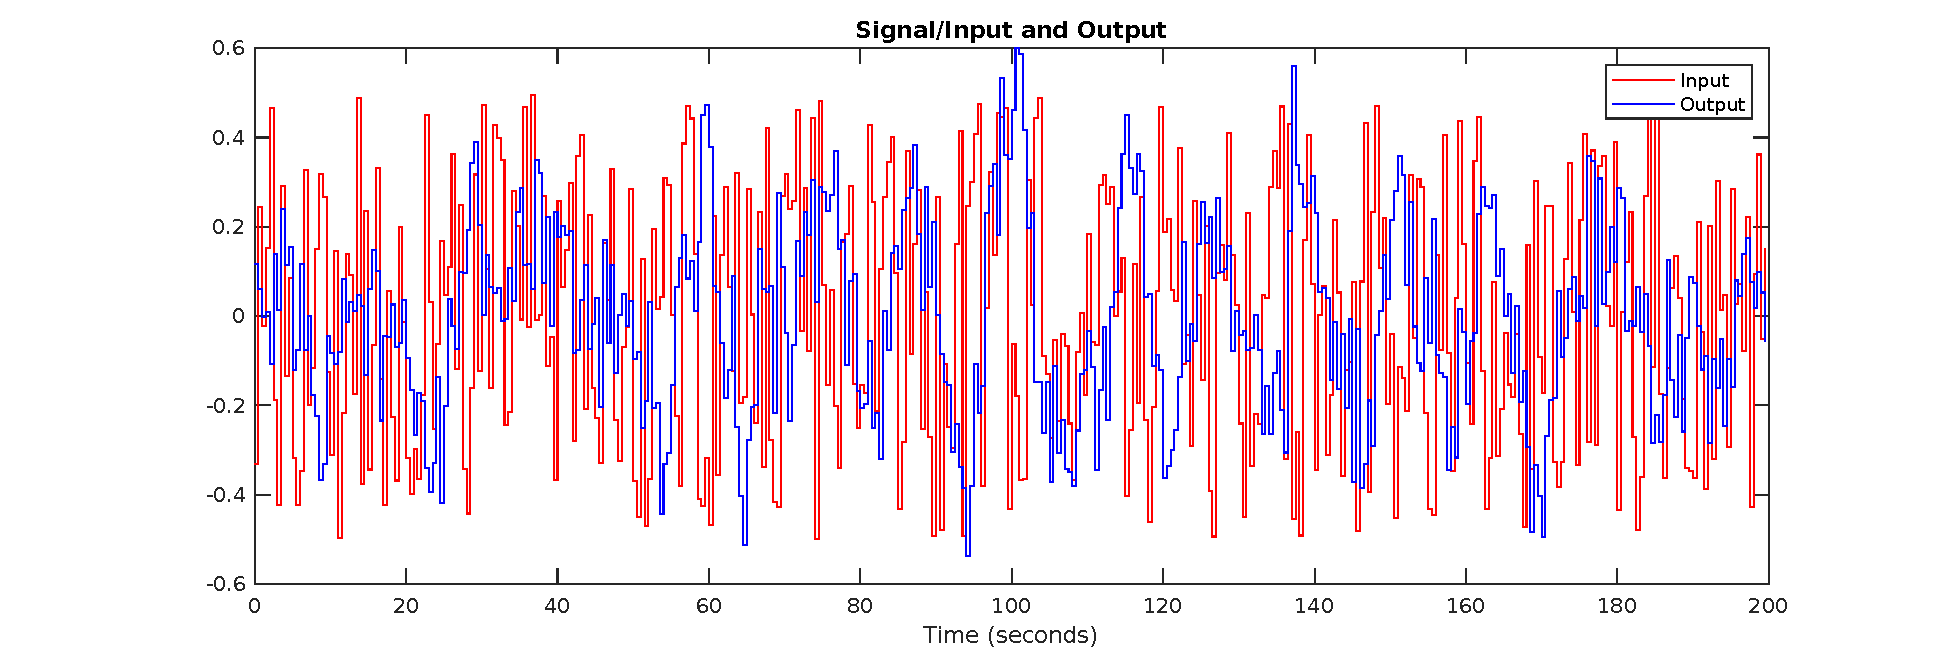
\includegraphics[height=5.5cm]{figures/input_output.pdf}
	\caption{Random input signal and output of the system}
	\label{fig:inout}
\end{figure}
Afterwards we can identify the discrete impulse response using the convolution relation
\begin{equation}
	y(k) = \sum\limits_{j=0}^{k} g(j)u(k-j) \text{ for } k=0,1,2,.. 
\end{equation}
or in a matrix form
\begin{equation}
	Y = U \Theta\, .
\end{equation}
Here, $U$ is an asymmetric (lower) triangular Toeplitz matrix.
Then, $\Theta$ can be calculated using
\begin{equation}
	\Theta = U^{-1} Y.
\end{equation}
However, this approach does not lead to a good solution as the matrix $U$ is poorly conditioned and very close to singular.
Therefore, the inversion is highly numerically unstable and we do not get a proper result for the discrete impulse response as shown in Figure~\ref{fig:originalimpulse}.

In order to fix the numerical problem, we shorten the total length of the impulse response by assuming $g(k) = 0$ for $k \geq K$ and we obtain $Y = U_{K} \Theta_{K}$ by removing the last $N-K$ columns of $U$ and the last $N-K$ rows of $\Theta$. 
This equation can be solved in the least squares sense using the Moore-Penrose pseudo inverse $U_{K}^+$ of $U_{K}$
\begin{equation}
	\Theta_{K} = (U^{T}_{K} U_{K})^{-1} U^{T}_{K} Y = U_{K}^{+} Y.
\end{equation}
In MATLAB we can compute the least squares solution by simply using the backslash operator.
As the true impulse response is approximately zero after $75 s$, we decided to set $K = 150$. Thus, the obtained impulse response can be seen in Figure~\ref{fig:impulseresponse}. The result is similar to the true impulse response of the signal, which we compute using the \verb|impulse| command in MATLAB.
Note that we of course do not know the length of the impulse response for arbitrary systems to be identified. 
Here, other methods to determine the main time constants or systematic evaluation of different target lengths $K$ must be employed.
Listing~\ref{lst:numdec} shows our implementation in MATLAB.
\matlabcode{../matlab/ce1/estimate_impulse_response_numdec.m}{Estimator of the impulse response via numerical deconvolution in MATLAB.}{lst:numdec}
\begin{figure}[h]
	\centering
	\begin{subfigure}{.49\textwidth}
		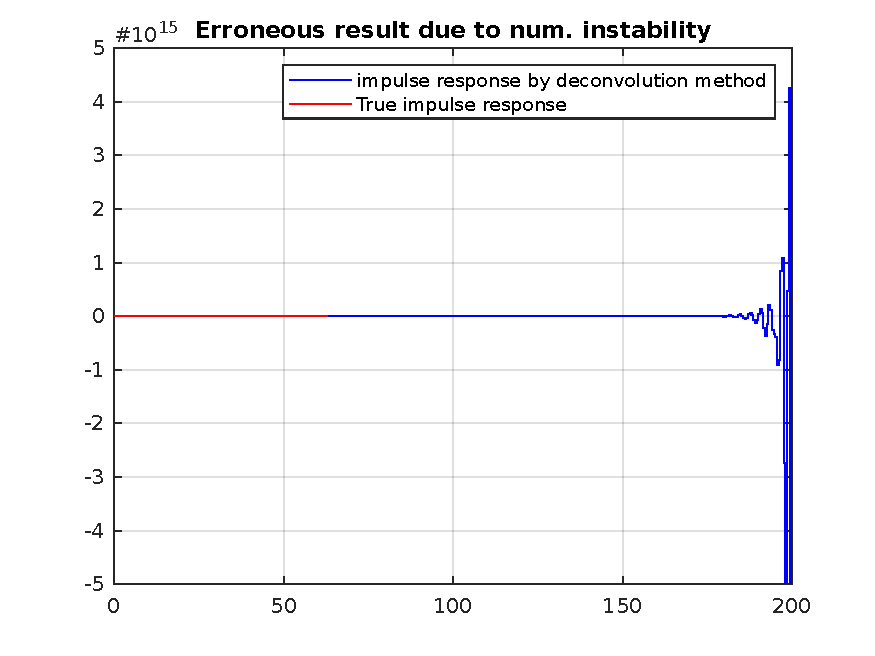
\includegraphics[width=\textwidth]{figures/original_impulse_response.pdf}
		\subcaption{Poor estimate of the impulse response due to the inversion of the poorly conditioned input matrix.}
		\label{fig:originalimpulse}
	\end{subfigure}
	\begin{subfigure}{.49\textwidth}
		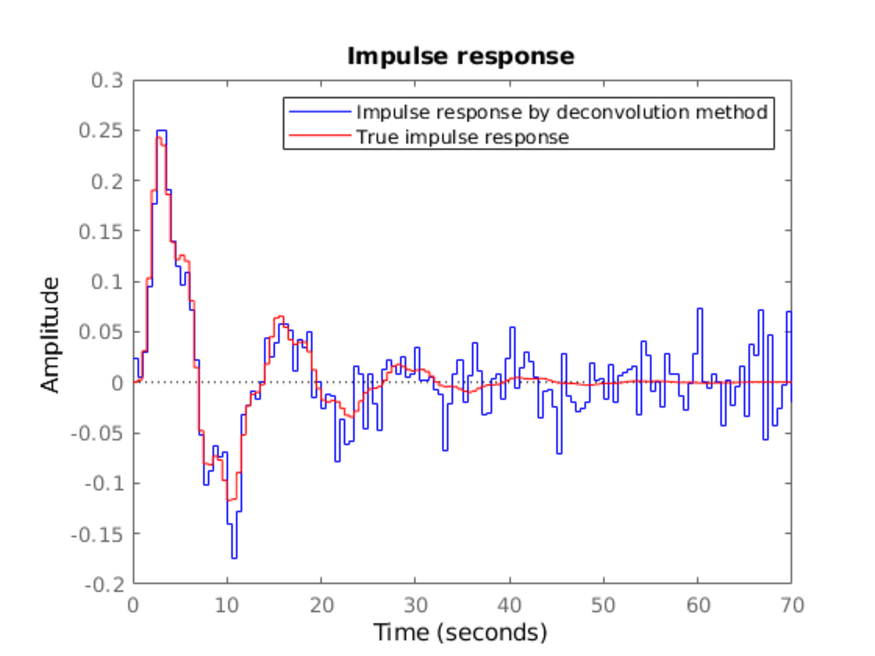
\includegraphics[width=\textwidth]{figures/impulse_response.pdf}
		\subcaption{Better estimate of the impulse response by constraining the length of the discrete finite impulse response.}
		\label{fig:impulseresponse}
	\end{subfigure}
	\caption{Impulse response by deconvolution method with random input signal}\label{fig:deconvolution}
\end{figure}

We get a 2-norm of the error vector as
\begin{equation}\label{eq:2-norm}
	E(\hat{g}) = \sqrt{\sum\limits_{k=0}^K \left(g(k) - \hat{g}(k)\right)^2}
\end{equation}
of $E(\hat{g}) = 0.22$.

\clearpage
\newpage
\section{Impulse Response by Correlation Approach}
We generate a PRBS signal with $4$ periods in a $7$ bit shift register model.
Afterwards, the PRBS signal is applied to the system.
First we compute the cross-correlation between the input and the output signal $R_{uy}(h)$ and the auto-correlation of the input signal $R_{uu}(h)$ using the previously implemented \texttt{intcor} function and MATLAB's \texttt{xcorr} function. The results are shown in Figure~\ref{fig:cross_correlations}.
\begin{figure}[h]
	\centering
	\begin{subfigure}{0.6\textwidth}
		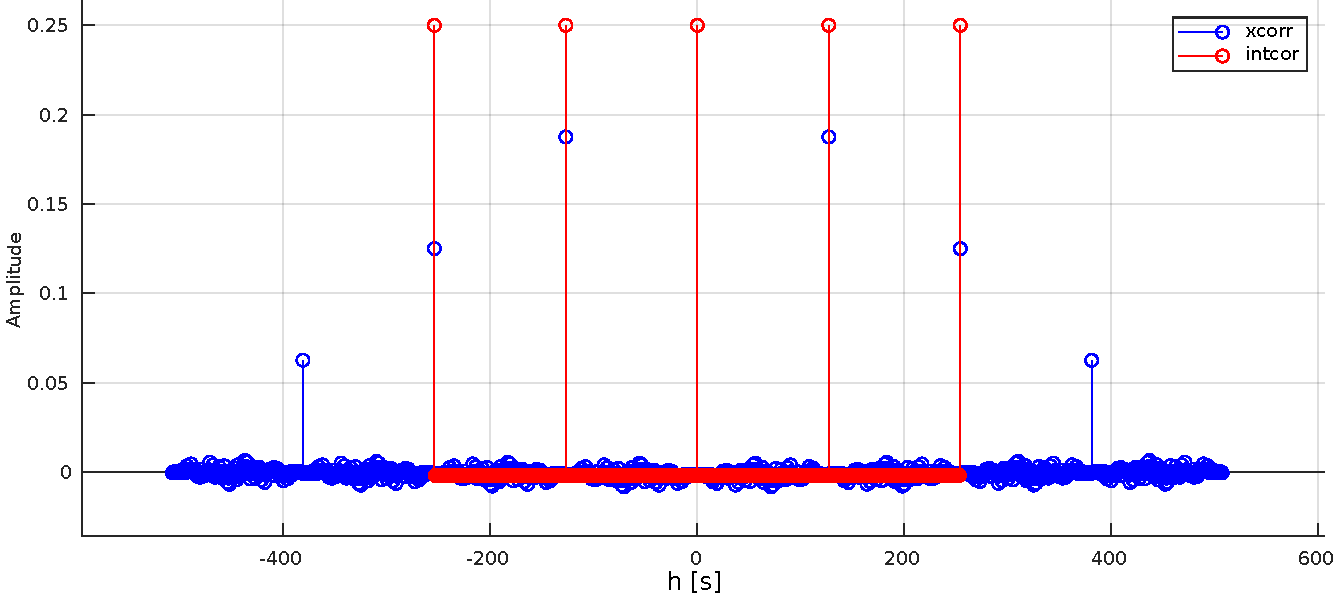
\includegraphics[width=\textwidth]{figures/ac.pdf}
		\subcaption{Auto-correlation $R_{uu}(h)$}
		\label{fig:cc_ac}
	\end{subfigure}
	\begin{subfigure}{0.6\textwidth}
		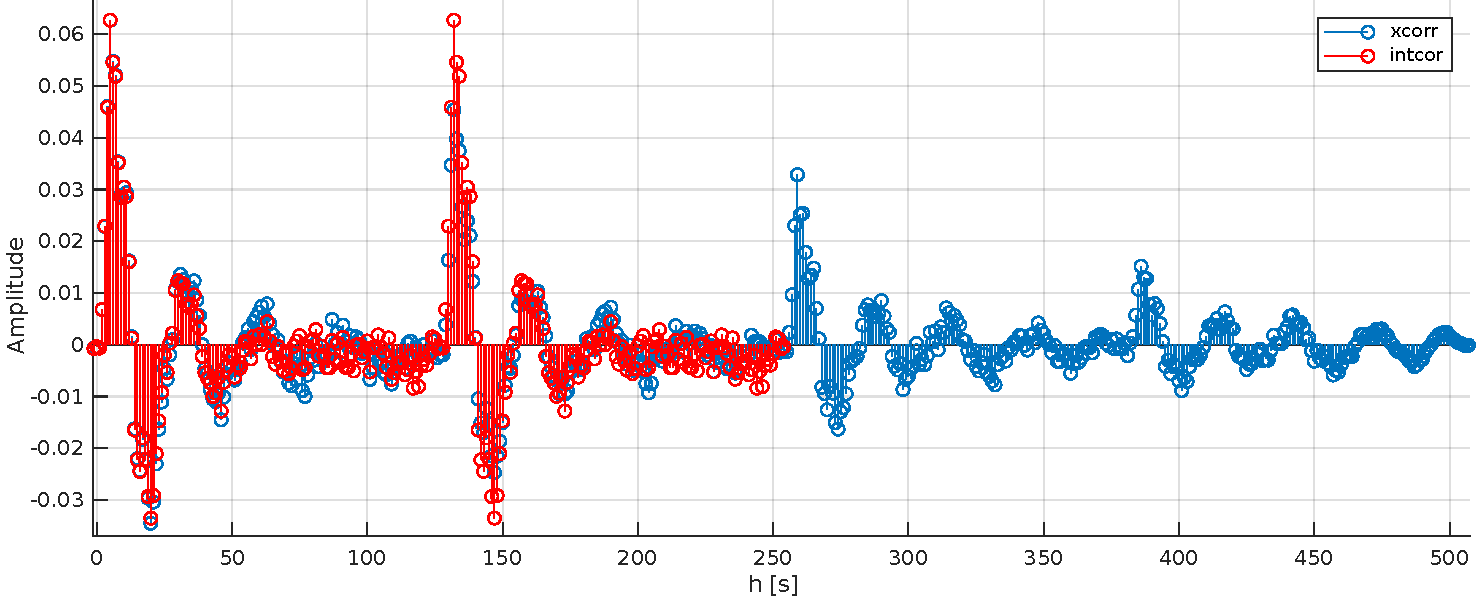
\includegraphics[width=\textwidth]{figures/cc.pdf}
		\subcaption{Cross-correlation $R_{yu}(h)$, (zoomed and truncated)}
		\label{fig:cc_cc}
	\end{subfigure}
	\caption{Correlation signals computed from input and output signal.}\label{fig:cross_correlations}
\end{figure}

The function \texttt{intcor} and \texttt{xcorr} yield the same results at $0$, but different results for the remaining values on the time-axis.
Generally, if $N$ is the signal length, \texttt{intcor} provides a correlation signal with a length of $N+1$ for $N$ even and $N+3$ for $N$ odd.
MATLAB's implementation yields a significantly longer signal and the correlation sum is weighted by some function of $h$.
Because of that, for $h\neq0$ MATLAB's \texttt{xcorr} shows a non-constant value for the PRBS auto-correlation while \texttt{intcor} does.
Figure~\ref{fig:correlation_impulse_responses} shows the resulting impulse responses in comparison to the ground truth.
We additionally compare the result of the simplified algorithms for white input signals.
As PRBS is not exactly white, we get lower performance for the simplified version and we have to apply numerical deconvolution to improve.
We implement the different approaches in the same function, an optional parameter allows to choose one of the methods. 
Our implementation is presented in Listing~\ref{lst:corr_approach}.
\begin{figure}[h!]
	\centering
	\begin{subfigure}{0.49\textwidth}
		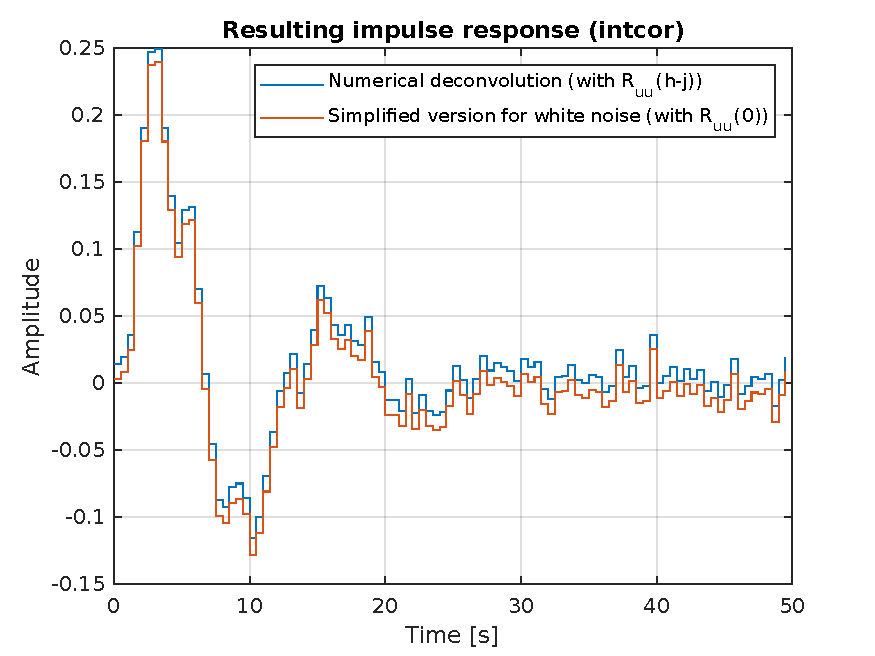
\includegraphics[width=\textwidth]{figures/impulse_response_intcor.pdf}
		\subcaption{Resulting impulse response using intcor.}
		\label{fig:impulse_response_intcor}
	\end{subfigure}
	\begin{subfigure}{0.49\textwidth}
		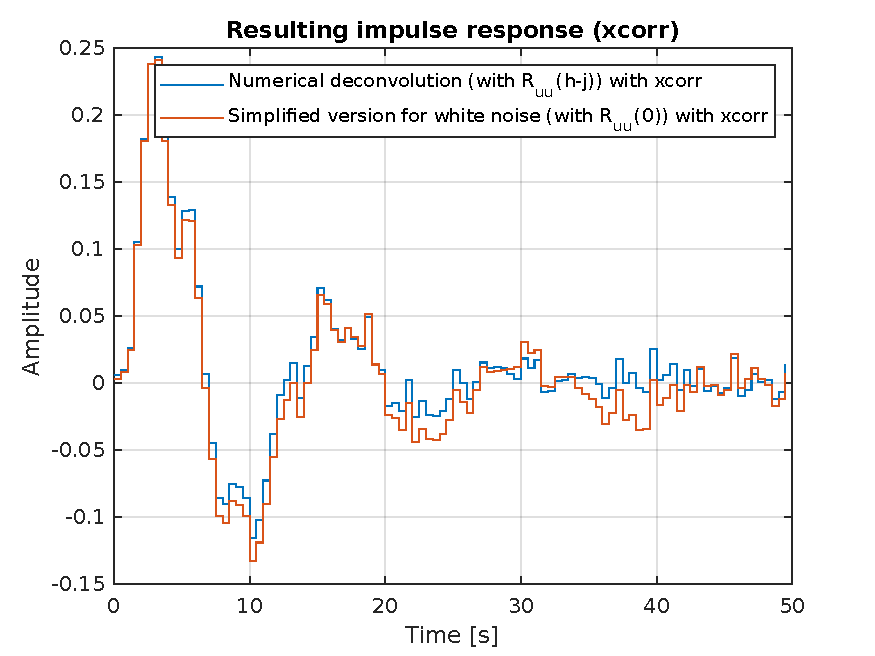
\includegraphics[width=\textwidth]{figures/impulse_response_xcorr.pdf}
		\subcaption{Resulting impulse response using xcorr.}
		\label{fig:impulse_response_xcorr}
	\end{subfigure}
	\begin{subfigure}{\textwidth}
		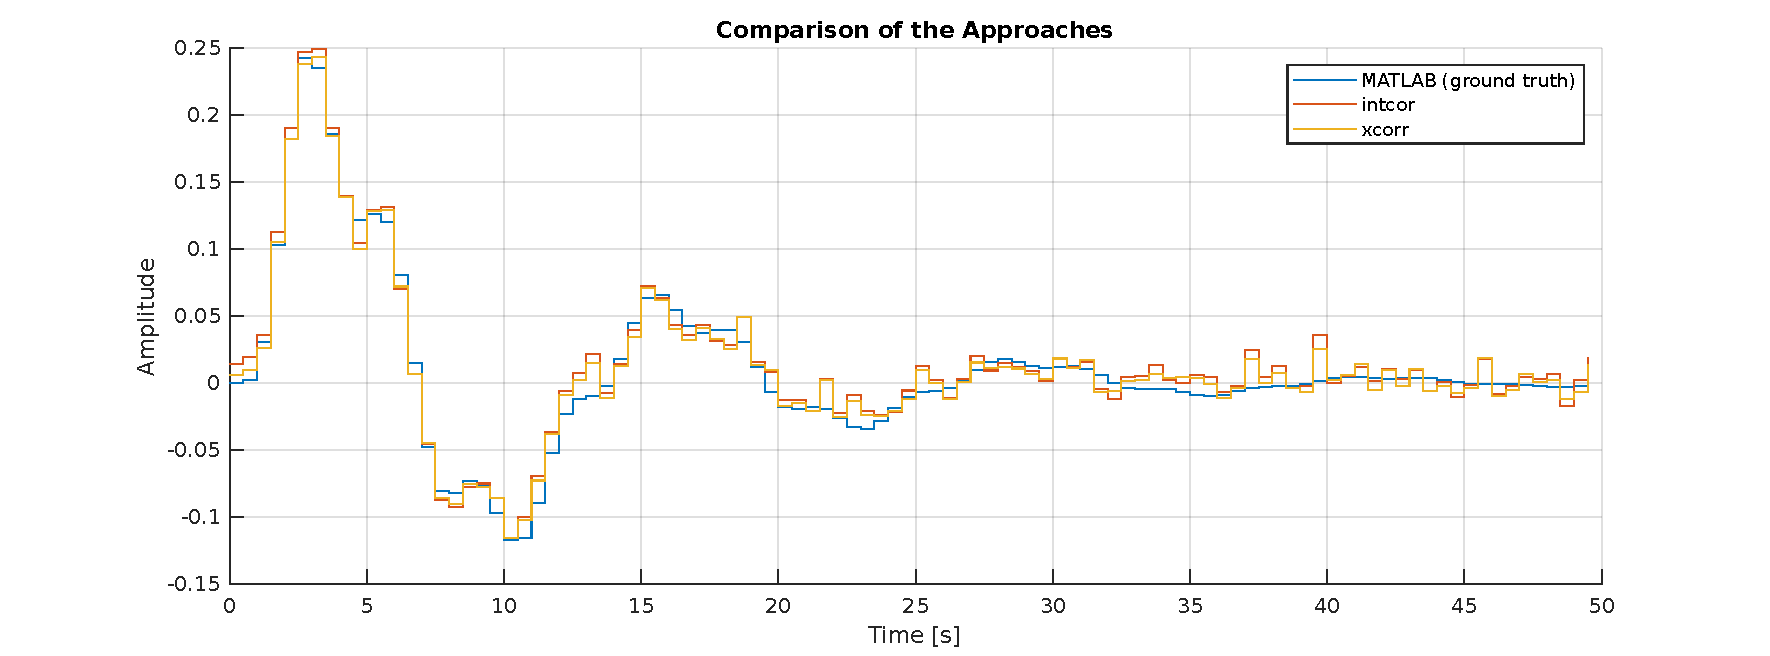
\includegraphics[width=\textwidth]{figures/impulse_response_comparison.pdf}
		\subcaption{Comparison with ground truth impulse reponse.}
		\label{fig:impulse_response_comparison}
	\end{subfigure}
	\caption{Comparison of the identified impulse response with the ground truth.}\label{fig:correlation_impulse_responses}
\end{figure}

Table~\ref{tab:correlation_appraoch_errors} shows the 2-norm of the errors between ground truth impulse response and the estimated results.
The 2-norms of the errors are computed based on \eqref{eq:2-norm}.
We additionally compare the result to the estimate of the numerical deconvolution algorithm developed in the previous section.
Note that, in contrast to the previous section, we now apply a PRBS signal instead of random white noise to the system.
We observe that the error of the numerical deconvolution approach is significantly smaller (approx. half as large) than in the previous section. 
As we use the same impulse reponse length $K$, the smaller error is due to the better eligible PRBS signal.
The comparison shows that the correlation approach with the \texttt{xcorr} correlation function creates the lowest error, while the correlation approach with the \texttt{intcor} function performs worst.
The performance of the previous numerical deconvolution of the input and output signals directly is between the new approaches of this section.
\begin{table}[h]
	\centering
	\begin{tabular}{l|c}
	\hline
	\hline
	\textbf{Approach} & \textbf{2-norm of error}\\
	\hline
		correlation approach using \texttt{intcor} & $0.13$ \\
		correlation approach using \texttt{xcorr} & $0.10$ \\\hline
		numerical deconvolution (1.\ref{section:numdec}) & $0.12$\\
	\hline
	\hline
	\end{tabular}
	\caption{Errors of the estimates of the impulse responses compared to the ground truth impulse response obtained by the MATLAB command. We compare the correlation approach algorithm for the correlation functions \texttt{intcor} and \texttt{xcorr} as well as the numerical deconvolution approach from the previous section.}
	\label{tab:correlation_appraoch_errors}
\end{table}

\matlabcode{../matlab/ce1/estimate_impulse_response_corr.m}
{Estimator of the impulse response via the correlation approach.}
{lst:corr_approach}

\newpage
\section{Frequency Domain Identification using a Periodic Signal}
In this task we want to use the Fourier analysis method to identify the frequency response of our model shown in Figure~\ref{fig:testmodel}. 
For the frequency domain identification we use $8$ periods of a PRBS signal generated by a $8$-bit shift-register.
Consequently, our total signal length is $N=2040$. The sampling frequency is at $\SI{2}{\hertz}$.
In order to get a good trade off between the resolution of the estimates (samples per period $M = 2^n -1$) and the impact of measurement errors (number of periods $p$) we decide to choose a signal with 8 periods ($p=8$) in a 8 bit ($n=8$) shift register.

First, we compute the Fourier transform of the input and the obtained output signal of our system using the \texttt{fft} command in MATLAB for each period. To reduce the measurement error we average the Fourier series coefficients but we ignore the first period
\begin{align}\label{eq:fft_average}
	 Y(n) = \frac{1}{p}\sum\limits_{i=2}^p Y_i (n) \quad \quad n = 1,2,\ldots,M
 \intertext{and} 
	U(n) = \frac{1}{p}\sum\limits_{i=2}^p U_i (n) \quad \quad n = 1,2,\ldots,M .
\end{align}
In addition, we calculate the frequency response $ G(e^{j \omega_n}) = Y(n)/ U(n)$. 
The results can be seen in Figure ~\ref{fig:ffts_diff}.
In order to determine the effect of noise to the frequency response, we compare the spectra of the system response to a PRBS signal and to a constant-zero input.
We can observe, that for frequencies higher than $\approx 2.5\frac{rad}{s}$ the signal is hidden in the noise and consequently we expect a poorer identification result in the frequency range higher than $\omega = 2.5\frac{rad}{s}$.

\begin{figure}[h!]
	\centering
	\begin{subfigure}{0.49\textwidth}
		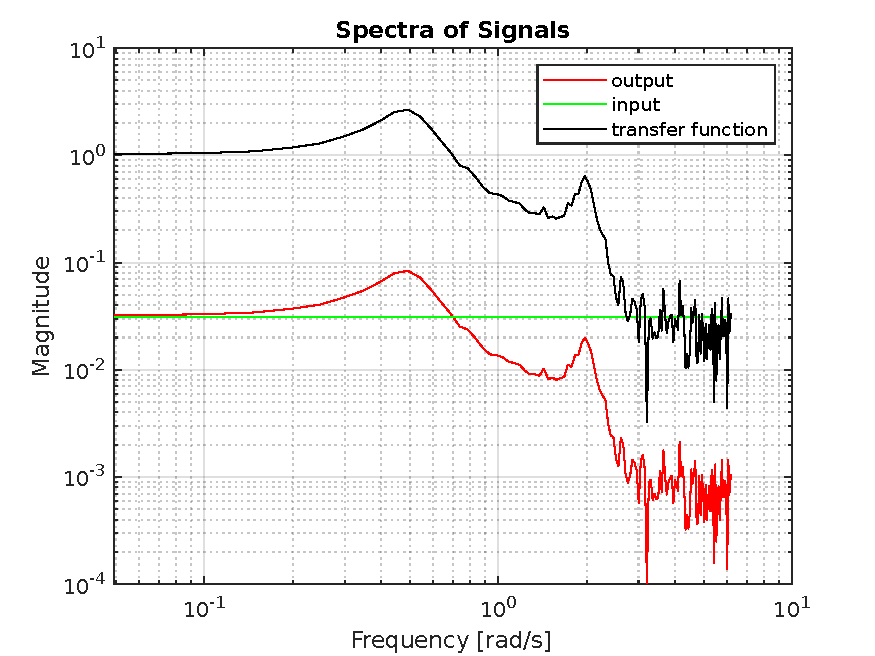
\includegraphics[width=\textwidth]{figures/ffts.pdf}
		\subcaption{input signal $U$, the output signal $Y$ and the transfer function $G$}\label{fig:ffts_diff}
	\end{subfigure}
	\begin{subfigure}{0.49\textwidth}
		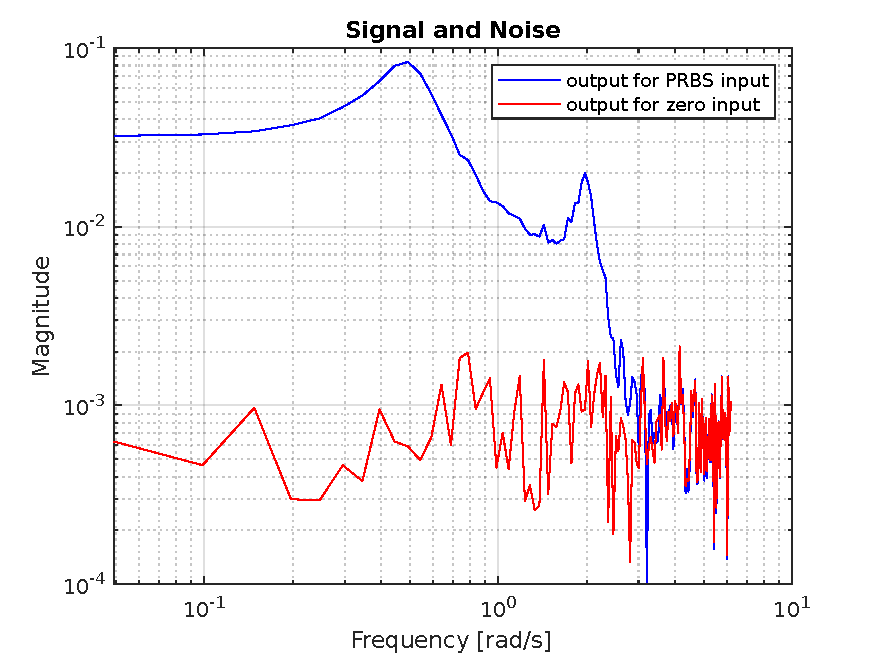
\includegraphics[width=\textwidth]{figures/ffts_snr.pdf}
		\subcaption{output signal for PRBS input and zero input}\label{fig:ffts_snr}
	\end{subfigure}
	\caption{Spectra of different signals. On the left we show the spectra of the input and output signals as well as the transfer function when applying the PRBS signal to the system. On the right we apply two different signals, a PRBS signal and a constant-zero signal, to the system and show the spectra of the system response. We can observe, that for high frequencies the system frequency response hides in the noise.}
\end{figure}
Afterwards we compute the frequency vector for one period
\begin{equation}\label{eq:f_vector}
	\left[ 0, \frac{\omega_s}{M},\frac{2\omega_s}{M}, \ldots, \frac{(M-1)\omega_s}{M} \right] .
\end{equation}
This vector is then used to generate a frequency-domain model using the MATLAB \texttt{frd} command. 
Finally, we compare the obtained Bode diagram of the identified model with the true one. Figure ~\ref{fig:resp_noiseless} shows the frequency response without noise. 
As we use a periodic signal, the truncation error is suppressed and the identified model approaches the true one (neglecting numerical errors) exactly. 
Figure ~\ref{fig:resp_noise} shows the frequency response applying a PRBS signal with the noise block switched on.
As we predicted based on the spectra of the output signals in Figure~\ref{fig:ffts_snr}, the estimated frequency response becomes poor for frequencies higher than $\approx 2.5 \frac{rad}{s}$.
\begin{figure}[h]
	\begin{subfigure}{0.45\textwidth}
		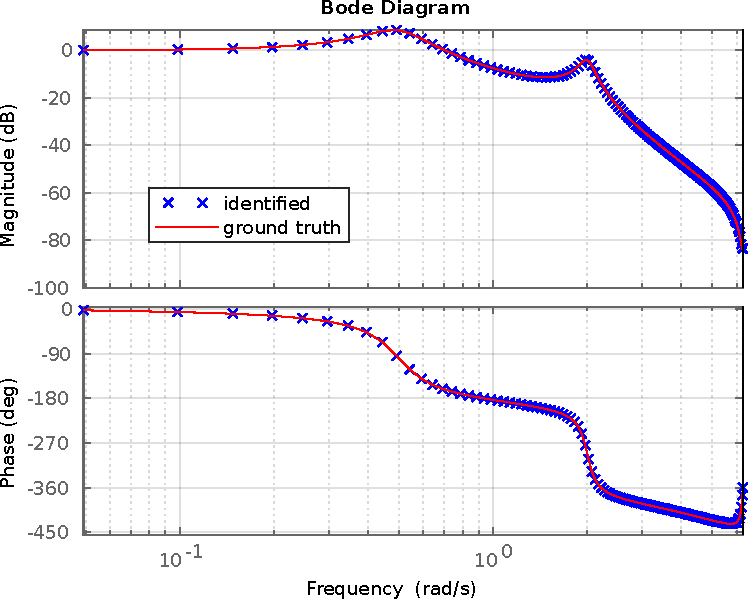
\includegraphics[width=\textwidth]{figures/resp_nonoise.pdf}
		\subcaption{Identified frequency response and true response with noise block switched off.}
		\label{fig:resp_noiseless}
	\end{subfigure}
	\hspace*{0.05\textwidth}
	\begin{subfigure}{0.45\textwidth}
		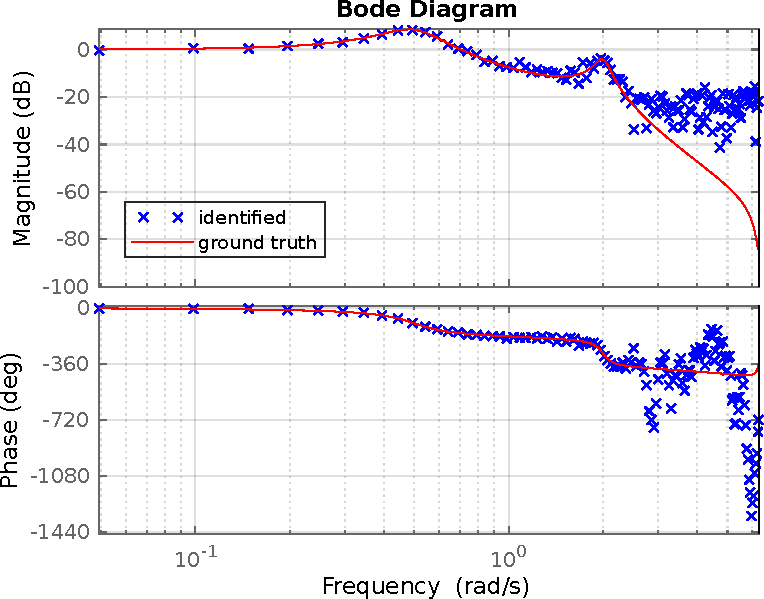
\includegraphics[width=\textwidth]{figures/resp_noise.pdf}
		\subcaption{Identified frequency response and true response with noise block switched on.}
		\label{fig:resp_noise}
	\end{subfigure}
	\caption{Comparison of the frequency response of the identified model with the true one}\label{fig:f_resp}
\end{figure}
\matlabcode{../matlab/ce1/estimate_frequency_response.m}
{{Compute the frequency response of the system to be identified using an average of Fourier transforms of each period. The first period is skipped as we wait for transience to vanish. Additionally, the frequency vector is computed.}}
{lst:freq_resp}

\clearpage
\section{Frequency Domain Identification using a Random Signal}

In contrast to the previous section, we now use a complete (non-periodic) random signal.
The signal should be white and should have a high energy in order to excite as much frequencies as possible. 
For Gaussian noise, samples are more likely to be close to zero than farer away. Therefore, the energy of a Gaussian signal is quite low.
Furthermore, we have a saturation block in the system.
Gaussian noise has no real maximum value on the samples generated, sample just become less likely, when their magnitudes become bigger.
It would be required to squeeze the Gaussian noise back into the $[-0.5, 0.5]$ interval, which would also change the power spectrum.
We therefore choose a uniform distribution as we do not need power-spectrum density shaping postprocessing on the samples generated.
As we want high energy, we choose a binary discrete random process with the two states $-0.5$ and $0.5$.
The power spectrum of the signal generated by this process is flat and has the highest energy.
Additionally, as the distribution is uniform, the signal has zero-mean.

This time, we estimate the frequency response of the system using the spectral analysis method.
Consider the correlation-based approach relation
\begin{equation}
	R_{yu}(h) = g(h) * R_{uu}(h) \underset{\mathcal{F}}{\Rightarrow} \Phi_{yu}(\omega) = G(e^{j \omega}) \Phi_{uu}(\omega)\, ,
\end{equation}
which yields
\begin{equation}
	G(e^{jw}) = \frac{\Phi_{yu}(\omega)}{\Phi_{uu}(\omega)}\, ,
\end{equation}
where $\Phi_{yu}(\omega)$ and $\Phi_{uu}(\omega)$ denote the Fourier transform of the cross-correlation $R_{yu}$ and the auto-correlation $R_{uu}$, respectively.
Further, the correlation functions can be multiplied by a windowing function in order to remove the noise due to the high variance of the estimates of the correlation function for large $h$.
Figure~\ref{fig:cross_corr_windowed} shows our implementation of the windowing of the correlation signals.
We parametrize the window shape by the parameter $M$, which specifies the number of samples to keep in both direction of the $0$ such that the total window has a length of $2M+1$. As the number of samples returned by our correlation function \texttt{intcor} is always odd, we can always guarantee that the maximum value of the window coincides with $h=0$.
\begin{figure}[h]
	\centering
	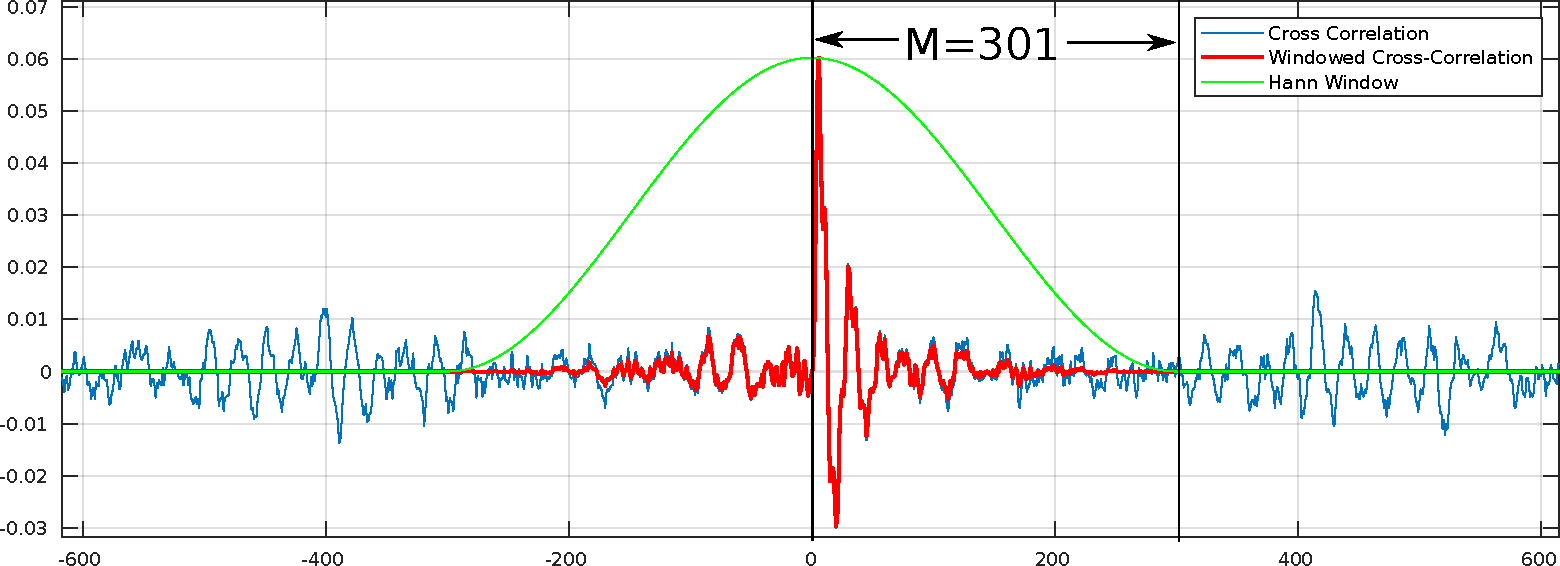
\includegraphics[width=\textwidth]{figures/windowed_cross_cor.pdf}
	\caption{Cross-correlation signal in windowed cross correlation signal.}
	\label{fig:cross_corr_windowed}
\end{figure}

Figure~\ref{fig:resp_spec_ana} shows the results for different window functions and window widths and Listing~\ref{lst:resp_spec_ana} shows the corresponding implementation.
We can observe, that the frequency response directly obtained without further processing like windowing or averaging is highly noise.
The windowed versions yield smoother results.
While a very narrow window leads to blurring of the details of the spectrum, a wider window increases the number of available fine details.
At the same time, noise also becomes more present increasing the width of the window.
Here, a setting of $M=301$ shows the best results, as it captures the peaks, but it is not as wiggly as the results for $M=1001$.
\begin{figure}[h]
	\centering
	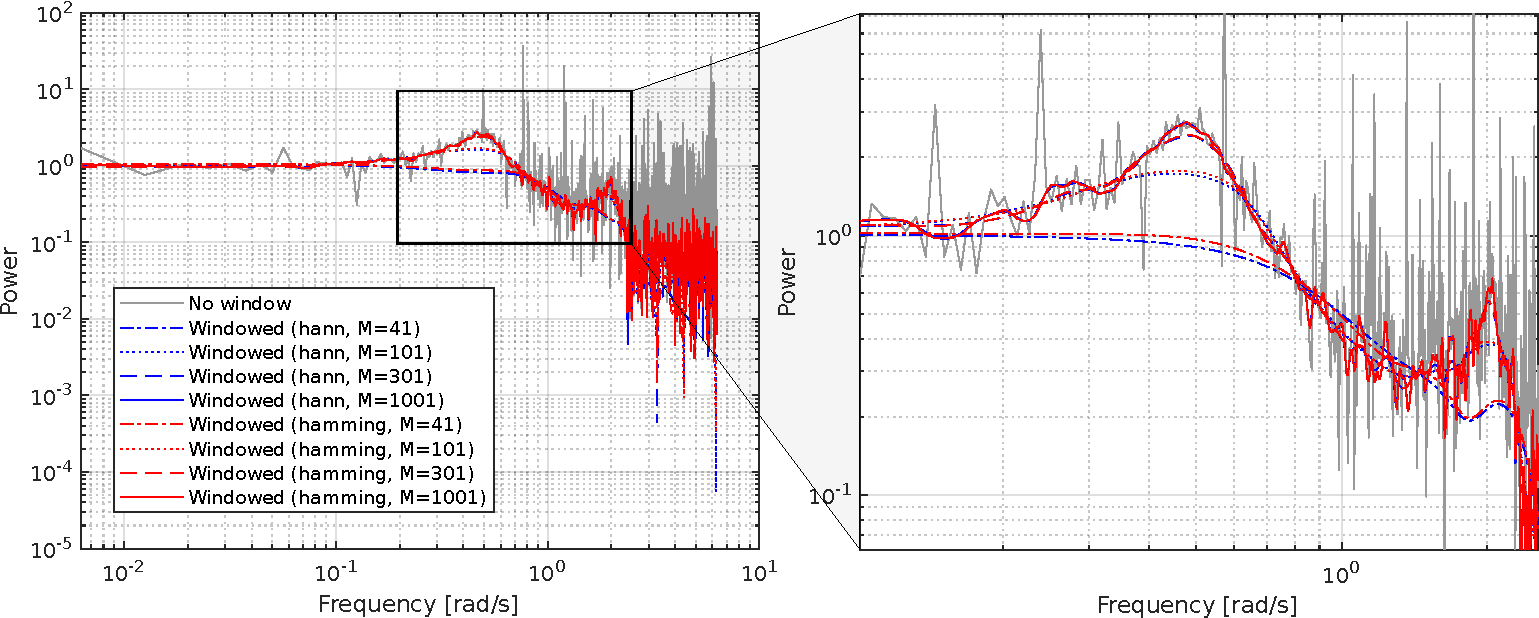
\includegraphics[width=\textwidth]{figures/freq_resp_spec_ana.pdf}
	\caption{Identified frequency response for different windows and window-sizes.}
	\label{fig:resp_spec_ana}
\end{figure}

After this, we also implement the averaging over multiple spectra splitting the available data into distinct groups.
We split the data into $m$ groups such that each group consists of $n = \left\lfloor\frac{N}{m}\right\rfloor$ samples.
On the one hand, increasing the number of groups promised that noise will average out.
On the other hand, we also loose frequency resolution increasing the number of groups.
Figure~\ref{fig:bode_final} shows the final results for the spectral analysis approach.
We compare the ground truth obtained from the transfer function directly with different methods in a Bode plot.
As in the previous section, the accuracy is very low for higher frequency, as the signal hides in the present noise.
In the higher frequency range, the signal is damped so much that the noise has higher power.
Even though, the averaged version of the frequency response without windowing shows better results that the non-averaged one, the windowed methods show better performance.
We achieve the best performance using a hann window with $M=301$ and using $m=2$ groups for averaging.
While there is no big difference visible in the magnitude plot, the phase plot shows better performance for the averaged version.
\begin{figure}[h]
	\centering
	\begin{subfigure}{\textwidth}
		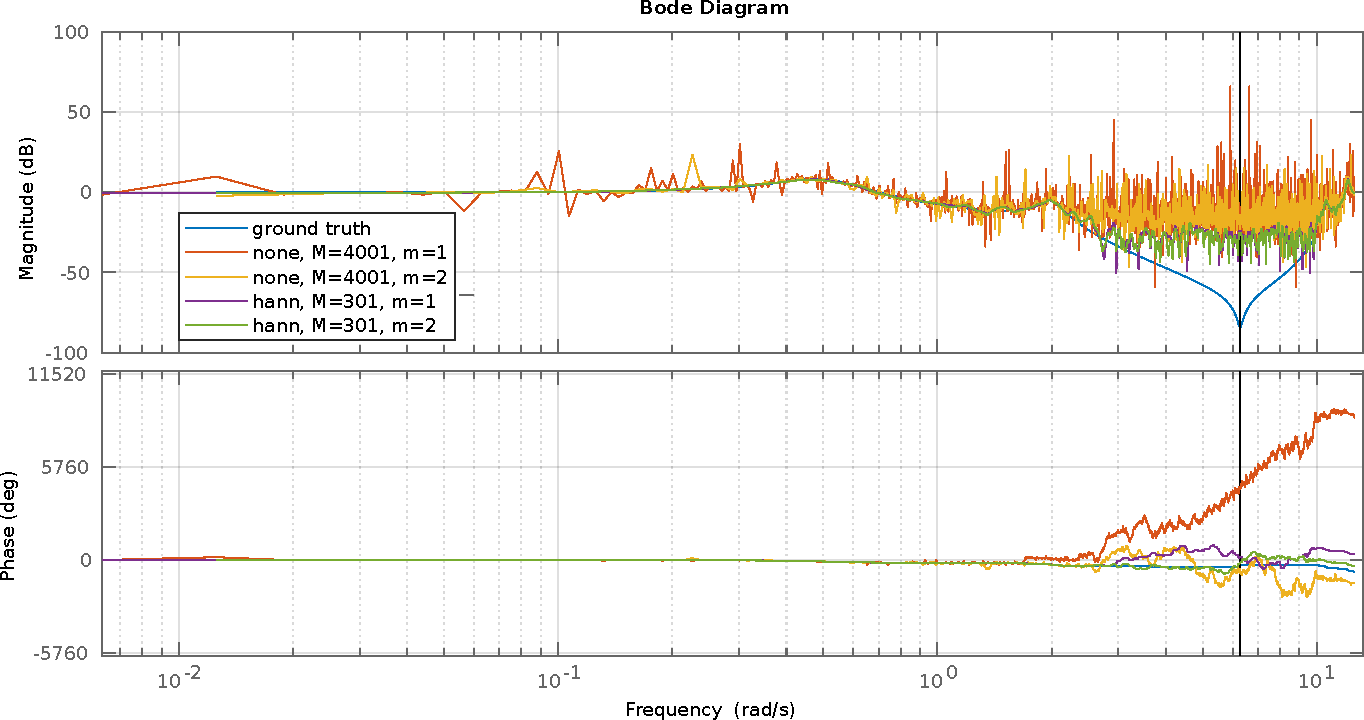
\includegraphics[width=\textwidth]{figures/bode_1_6_large.pdf}
		\subcaption{Bode diagram}
	\end{subfigure}
	\begin{subfigure}{\textwidth}
		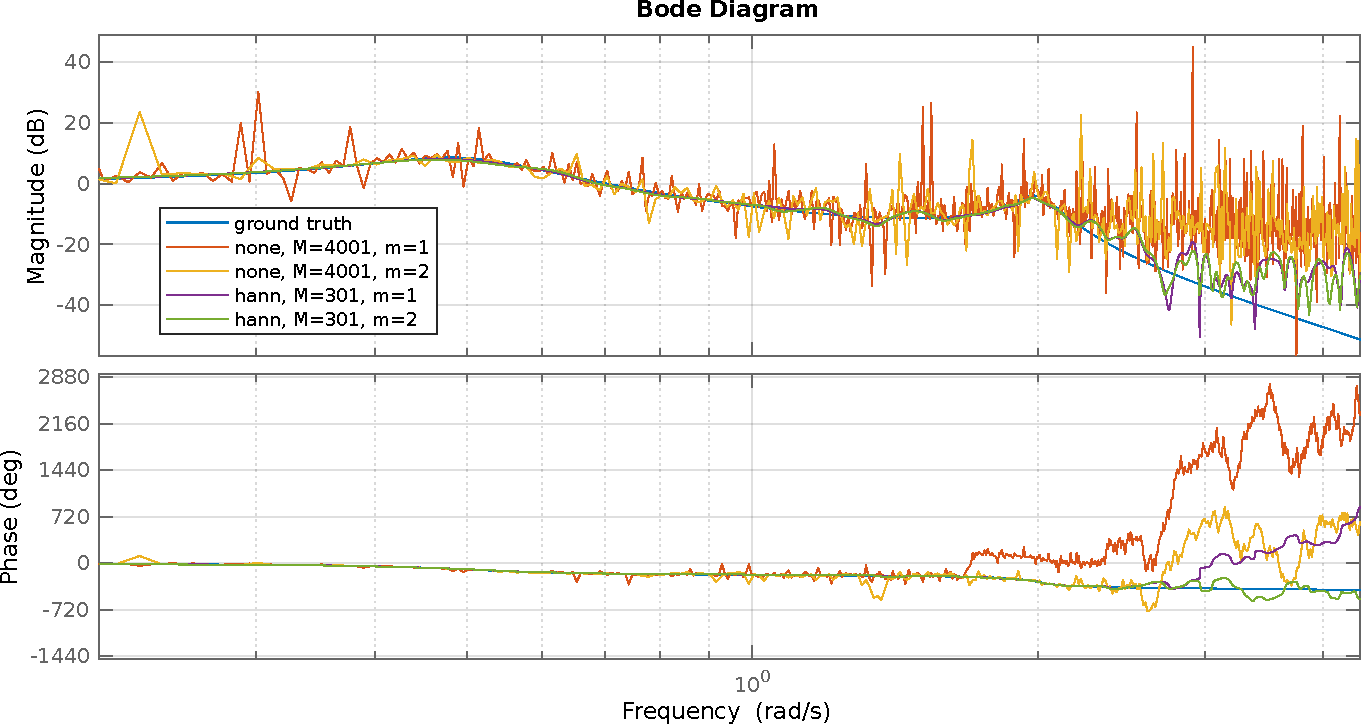
\includegraphics[width=\textwidth]{figures/bode_1_6.pdf}
		\subcaption{Bode diagram (zoomed)}
	\end{subfigure}
	\caption{Bode diagram comparing the ground truth frequency response and the identified frequency response obtained using different methods. In general, the methods using the window functions achieve better results. The best phase information is obtained using a hann-window and averaging over two groups.}
	\label{fig:bode_final}
\end{figure}

\matlabcode{../matlab/ce1/spectral_analysis.m}
{{Compute the frequency response of the system to be identified using the spectral analysis method. The function interface provides additional parameters for specifiying the (optional) window and the corresponding window-width. If no window parameters are given, no window is used.}}
{lst:resp_spec_ana}

\end{document}
